\section{Evaluation}
\label{sec: eval}

In this section, we evaluate the following questions regarding Meteor's design.

\begin{itemize}

\item To what extent data locality achieved through LAM decrease job time and bandwidth consumed?
\item What's the improvement in latency when BAWS is used on top of LAM?

\end{itemize}

For our evaluation, we use the Emulab testbed \cite{emulab}. Emulab gives us the ability to configure arbitrary network topologies and link bandwidths. In this initial evaluation, each node in our Emulab topology represents a datacenter and a link connecting two nodes represents a link in the wide-area. 
%In addition to relatively easier and quicker prototyping 
We plan to extend the setup to contain multiple nodes in a cluster as future work.  We have configured our environment in Emulab by installing Spark and its dependencies. Note that Spark requires the data to be stored on a shared filesystem, such as HDFS. To give our system this illusion while ensuring that data is accessed over the traffic-shaped links, we set up NFS servers at each node and disabled client-side caching. Each emulab node has 2GB RAM, and two Intel Xeon 3.00GHz processors.

For data, we use publicly available wikipedia data. The total size of our dataset is 4GB. We chose this size for fast prototyping, considering emulab's status as a highly shared and thus resource-constrained testbed. 
Each node has a split of the total data on its local storage. Our example query, unless otherwise stated, is 
`word count'. The size of each data block is 64MB. Unless otherwise stated, each data point is the mean of three runs.

\subsection{Job Latency and Bandwidth Usage for LAM}
For this experiment, we use a two-cluster `dumbbell' topology with each `cluster' containing two nodes, and
connected to the other cluster with a WAN link. Data is split equally between the two clusters. 
Figure~\ref{fig:job-time-localMap} shows how the job execution time changes as the link bandwidth is varied,  %This is compared against both nodes col-located, i.e., without communication over the WAN. 
with MapReduce/Spark  compared with Location-Aware Map (LAM). 
It clearly shows that the job runtime is very sensitive to the amount of available bandwidth between workers. The Spark runtime is improved by almost 68 \% when the available bandwidth is increased from 5 to 10 Mbps, with it further decreasing as the bandwidth is increased.  
In contrast, LAM achieves significantly better runtime even when the bandwidth is really small. This is expected since data locality is strictly enforced and hence no map input block travels over the WAN link. 
The slight decrease in runtime as the link bandwidth goes up is due to the fact that reduce input still
uses the link due to the all-to-all nature of the reduce phase. 

\begin{figure}[!ht]
\centering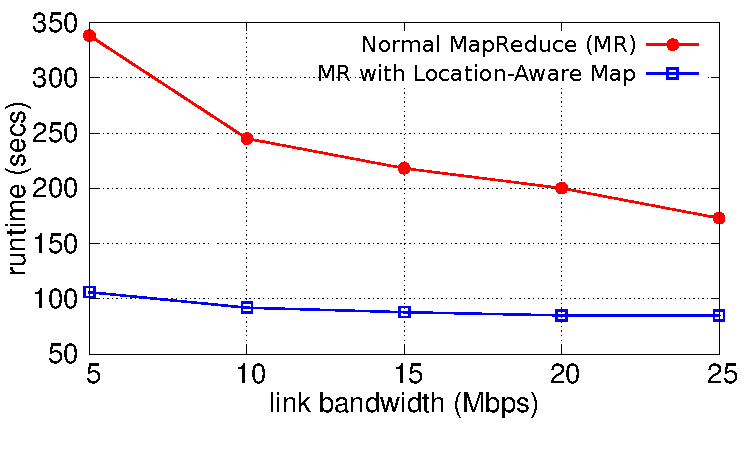
\includegraphics[width=\columnwidth]{figs/job-time-localMap.pdf}
\vspace{-1.2em}
\caption{Spark job execution time increases drastically as the wide area link bandwidth decreases. Latency 
for the Location-Aware Map is significantly better.}
\label{fig:job-time-localMap}
\vspace{.7em}
\end{figure}

\begin{figure}[!ht]
\centering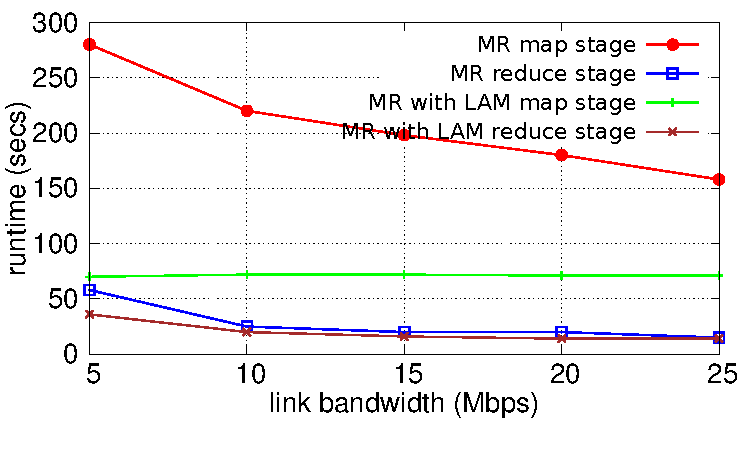
\includegraphics[width=\columnwidth]{figs/stage-time-localMap.pdf}
\vspace{-1.2em}
\caption{Enforcing data locality for the map stage makes map runtime constant no matter the available bandwidth.}
\label{fig:stage-time-localMap}
\vspace{.7em}
\end{figure}

Figure~\ref{fig:stage-time-localMap} splits the runtimes shown in Figure~\ref{fig:stage-time-localMap} into the individual map and reduce stages. It's evident that most of the improvement comes from enforcing strict data locality through LAM and hence make the map runtime independent of the link bandwidth. 

\subsection{Job Latency for BAWS}

To measure the effect of Bandwidth-Aware Work Stealing, we use a topology containing three nodes A,B,C, with every pair of nodes connected together. 
Again each node represents a data center and each link represents a WAN link. The overall dataset is of size 4.5GB, with splits of 0.5GB, 2GB and 2GB respectively. This skew will result in the node with the smallest split, i.e., A, finish its task queue first and enter work-stealing mode. To reduce complexity in the experiment, link A-B's capacity is always configured to be higher than A-C's, and hence A will steal work from B. We vary A-B's bandwidth.  
Figure \ref{fig:baws} shows the percentage job runtime decrease for BAWS scheduling compared with LAM scheduling as well as vanilla Spark, 
as a function of bandwidth on link A-B. The work-steal probability $p$ in this case is $0.5$. 
The red curve represents BAWS's improvements over LAM. As can be seen, the overall runtime actually \emph{increases} a little bit for very low bandwidth values.
This is because work-stealing results in node A running a map task stolen over the thin link. This will likely result in A still waiting for the data over the wire when B finishes the rest of its queue. As the bandwidth increases, this likelihood decreases and we start seeing the benefits of BAWS.
As can be seen, BAWS can gives us a 10-15\% speedup in job runtime over LAM. The blue curve represents BAWS's improvements over
Spark. Since BAWS is implemented on top of LAM, this is our combined system. As is evident again, the speedup is significant, and is most salient
for low bandwidths.


\begin{figure}[!ht]
\centering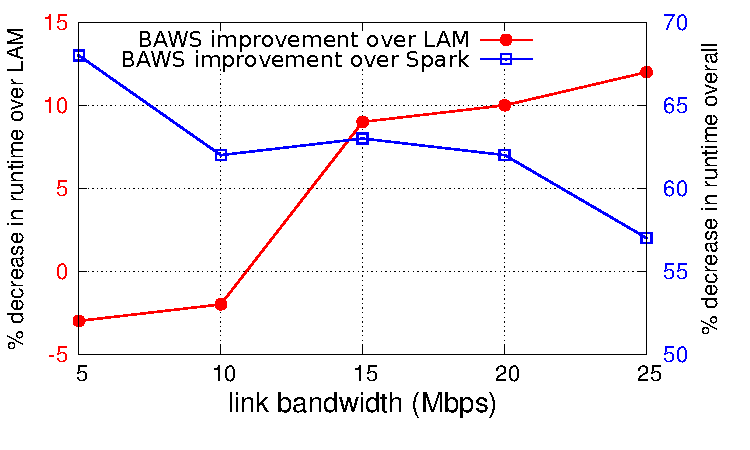
\includegraphics[width=\columnwidth]{figs/baws.pdf}
\vspace{-1.2em}
\caption{BAWS improves the job runtime even further than LAM unless the bandwidth is really low. The BAWS probability is this case 0.5}
\label{fig:baws}
\vspace{.7em}
\end{figure}

\subsection{Query result quality degradation for communication-avoiding iterative MapReduce}

To measure quality degradation on query result when using communication-avoiding iterative MapReduce (CAIM), we run an iterative PageRank algorithm on top of Meteor on a toy PageRank dataset containing thousands of pages. Our pagerank implementation makes use of consistent partitioning and combining in order to reduce unnecessary communication. We partition the input dataset into two roughtly even partitions and run the PageRank algorithm over 64 iterations. In our baseline, we run the PageRank algorithm by allowing inter-node communication at each step of the algorithm. We then run the PageRank algorithm by exponentially decreasing the number of iterations where inter-node updates are allowed. The \emph{communication avoidance rate} describes the ratio of MapReduce iterations where inter-node communication is disallowed. We evaluate quality degradation on the query result when only 32, 16, 8, 4, 2, and 1 inter-node updates are allowed during the execution of the PageRank iterative algorithm. Allowing only 1 inter-node update during the entire execution of the algorithm is equivalent to running PageRank independently on two nodes, and merging the PageRanks computed in the two sets at the end, by performing one pass of MapReduce on the union of the two partitions. 

We report the Normalized Root Mean Squared Error obtained when running PageRank using CAIM. We observe that performing only one cross-node update over 64 iterations yields an NRMSE above 5\%. Decreasing the communication-avoidance rate down to one cross-node update every 32 iterations results in an NRMSE below 3\%. Interesingly, further decreasing the communication avoidance rate has no impact on the NRMSE of the query results. 

We decided to look at a different error metric, which is the set intersection of the top K query results, which we will refer to as top-k error. Figure \ref{fig: CAIM} indicates that that reducing the communication-avoidance rate from 75\% down to 50\% greatly minimizes top-k error. This shows us that CAIM implemented in Meteor should in theory cut inter-node communication in half during the iterative phase of PageRank, while yielding acceptable query results. 

\begin{figure}[!ht]
\centering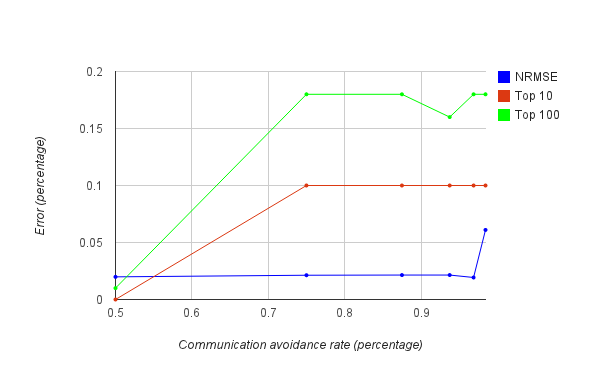
\includegraphics[width=\columnwidth]{figs/comm_avoid_PR.png}
\vspace{-1.8em}
\caption{Communication-avoiding iterative MapReduce (CAIM): we vary the communication-avoidance rate from 50\% to 98\% and report the NRMSE as well as the number of common entries in the top 10 and 100 pages produced by running PageRank with and without CAIM.}
\label{fig:CAIM}
\vspace{.7em}
\end{figure}

The caracterization of CAIM is still a work in progress. We wish to further explore the potential of CAIM for iterative queries: 

\begin{itemize}

\item Caracterize query result error on much larger PageRank data sets
\item Use ranking error metrics such as Kendall-Tau distance
\item Caracterize query result error on other iterative PageRank algorithms such as Kmeans
\item Measure the communication and run-time reduction of CAIM on Emulab once it is implemented as part of Meteor

\end{itemize}
